\documentclass[12pt,english]{article}
\usepackage[english]{babel}
\usepackage{graphicx}
\usepackage{amsmath}
\usepackage{multirow}
\usepackage{pgfplots}
\usepackage{subcaption}
\usepackage{amssymb}
\usepackage[hidelinks]{hyperref}
\usepackage{caption}
\usepackage{amsthm}
\usepackage{multicol}
\pgfplotsset{compat=1.16}
\usepackage{minted}
\usepackage{float}
\usepackage{titling}
\usepackage{soul}
\usepackage{listings}
\newenvironment{statement}{\fontfamily{ptm}\selectfont}{\par}
\usepackage{array}
\graphicspath{ {../img/} {./img}}
\selectlanguage{english}
\usepackage[nottoc]{tocbibind}
\usepackage[utf8]{inputenc}
\usepackage{graphicx}
\usepackage[a4paper,left=2cm,right=2cm,top=2.5cm,bottom=2.5cm]{geometry}
\RecustomVerbatimEnvironment{Verbatim}{BVerbatim}{}

\newmintedfile[matlabcode]{matlab}{
linenos=true,
tabsize=2,
breaklines=true,
}


\title{Evolutionary Algorithms}
\setlength{\droptitle}{10em}
\author{Carlos Sánchez Páez}

\makeindex
\begin{document}


\begin{titlepage}

\newlength{\centeroffset}
\setlength{\centeroffset}{-0.5\oddsidemargin}
\addtolength{\centeroffset}{0.5\evensidemargin}
\thispagestyle{empty}

\noindent\hspace*{\centeroffset}
\begin{minipage}{\textwidth}

\centering

\includegraphics[width=0.75\textwidth]{bme_logo.jpg}\\[1.4cm]

\textsc{ \Large Evolutionary Algorithms\\[4cm]}

\textsc{\Huge Homework}\\[0.75cm]

{\Large\bfseries Tenth task\\}
\end{minipage}

\vspace{8cm}
\noindent\hspace*{\centeroffset}
\begin{minipage}{\textwidth}
\centering

\textbf{Author}\\ {Carlos Sánchez Páez}\\
\texttt{http://www.github.com/csp98}\\[0.5cm]
\textsc{Budapest University of Technology and Economics}\\
\vspace{1cm}
\textsc{Academic year 2018-2019}
\end{minipage}
\end{titlepage}
\thispagestyle{empty}

\newpage


\begin{enumerate}

	\item
		\begin{statement}
		Write the gradient method algorithm in your favorite programming language, and test it for the $f(x,y)=x^2 + y^2$ function and for your own test-function (the two dimensional version of it).
		\begin{center}
			CHI5TC Rosenbrock function
		\end{center}
		\end{statement}
		I wrote the gradient method algorithm in \emph{Matlab}. The code is the following:
		\begin{figure}[H]
			\centering
			\matlabcode{gradient_method.m}
		\end{figure}
		The chosen parameters and the results are:
		\begin{figure}[H]
			\centering
			\begin{tabular}{|c|c|c|c|c|}
			\hline
				& \textbf{Initial point} & \textbf{Learning rate} & \textbf{Iterations} & \textbf{Result}\\
				\hline
				$f(x,y)=x^2+y^2$ & (6,6) & 0.01 & 1000 & $f(0,0)=0$ \\
				\hline
				Rosenbrock function & (6,6) & 0.0001 & 10000000 & $f(1,1)=0$\\
				\hline
			\end{tabular}
		\end{figure}

		\begin{figure}[H]
		    \centering
		    \begin{subfigure}[b]{0.45\textwidth}
		        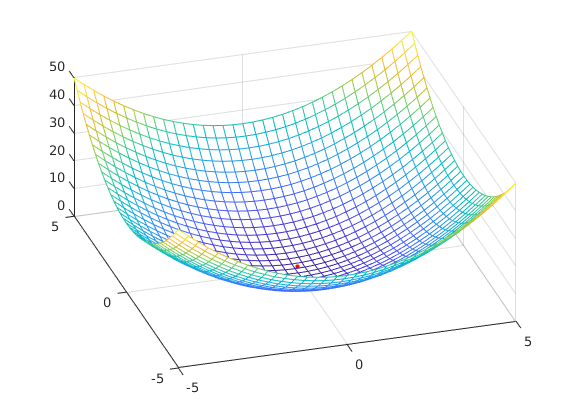
\includegraphics[width=\textwidth]{first}
		        \caption{$f(x,y)=x^2+y^2$}
		    \end{subfigure}
		    \begin{subfigure}[b]{0.45\textwidth}
		        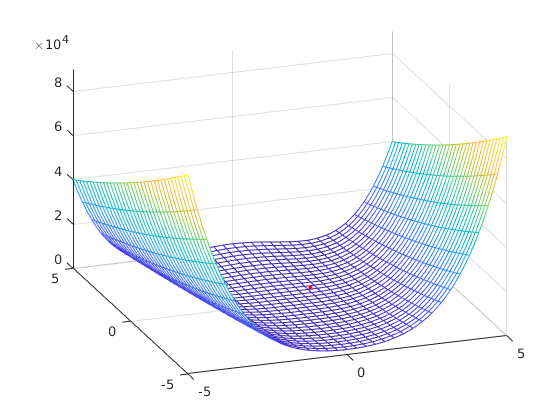
\includegraphics[width=\textwidth]{rosenbrock}
		        \caption{Rosenbrock function}
		    \end{subfigure}
		\end{figure}
		For the Rosenbrock function I had to desing an auxiliar function for the gradient, in order not to take very high symbolic variables that made the running time too big.
\end{enumerate}


\begin{thebibliography}{9}

\bibitem{Course Webpage}
Course Webpage
\\\texttt{http://math.bme.hu/~safaro/evolalgen.html}


\bibitem{Webpage4}
\texttt{https://tex.stackexchange.com/}


\end{thebibliography}


\end{document}
